\chapter{Входные и выходные данные}

Входные данные программы: путь к директории с html страницами полученных в рамках ЛР №4.

Выходные данные: файл, содержащий замеры необходимых времен, json файл, содержащий извлеченные данные в структурированном виде.
\clearpage

\chapter{Преобразование входных данных в выходные}

Для реализации указанной задачи был выбран язык C++~\cite{cpp}, т.~к. данный язык предоставляет возможность работать с динамической памятью с помощью контейнерных классов.

Для сохранения очередей задач перед каждой стадией конвейера был написан класс, представленный в листинге~\ref{lst:queue}. Указанный класс содержит также необходимые средства взаимоисключения для работы нескольких потоков с очередью одновременно. 
\begin{lstlisting}[caption={Класс очереди задач}, label=lst:queue]
template<typename T>
class task_queue {
public:
	void push(const T &elem) {
		tasks.push(elem);
	}
	T pop() {
		T top = tasks.front();
		tasks.pop();
		return top;
	}
	bool empty() {
		return tasks.empty();
	}
	condition_variable cv;
	bool pushed=false;
	mutex m;
	
private:
	queue<T> tasks;
};
\end{lstlisting}

В листингax~\ref{lst:read}~\ref{lst:parse}~\ref{lst:write}~\ref{lst:log} представлены различные классы для соответствующих стадий задач.
\clearpage
\begin{lstlisting}[caption={Класс задачи на этапе чтения файлов}, label=lst:read]
class read_task {
public:
	explicit read_task(string &file_1, string &file_2) : filename_1(file_1), filename_2(file_2),
	uuid(boost::lexical_cast<string>(
	boost::uuids::random_generator()())) {
		clock_gettime(CLOCK_MONOTONIC, &times["read_queue_push"]);
		cout << uuid << " " << "created\n";
	}
	vector<string> process();
	string get_uuid() { return uuid; }
	map<string, timespec> times;
private:
	string filename_1, filename_2;
	const string uuid;
};

vector<string> read_task::process() {
	setlocale(LC_ALL, "Russian");
	clock_gettime(CLOCK_MONOTONIC, &times["read_queue_start"]);
	std::ifstream file;
	file.open(filename_1, ios_base::in);
	
	std::string html_content((std::istreambuf_iterator<char>(file)), std::istreambuf_iterator<char>());
	file.close();
	file.open(filename_2, ios_base::in);
	string url;
	file >> url;
	file.close();
	clock_gettime(CLOCK_MONOTONIC, &times["read_queue_pop"]);
	return {html_content, url};
}
\end{lstlisting}

\clearpage
\begin{lstlisting}[caption={Класс задачи на этапе обработки содержимого файла}, label=lst:parse]
class parse_task {
public:
	explicit parse_task(vector<string> &values, string uuid_, const map<string, timespec> &old_times) : times(
	old_times), content(values), uuid(std::move(uuid_)), complete(true) {
		clock_gettime(CLOCK_MONOTONIC, &times["parse_queue_push"]);
	}
	string get_uuid() { return uuid; }
	task_dto process(); //returns JSON
	bool is_complete() { return complete; };
	map<string, timespec> times;
private:
	string search_for_recipe_detail_picture(GumboNode *node);
	vector<map<string, string>> search_for_ingredients(GumboNode *node);
	vector<string> search_for_recipe_steps(GumboNode *node);
	string search_for_title(const string &input);
	vector<string> content;
	const string uuid;
	bool complete;
};

task_dto parse_task::process() {
	clock_gettime(CLOCK_MONOTONIC, &times["parse_queue_start"]);
	task_dto result;
	result.uuid = uuid;
	result.url = content[1];
	GumboOutput *output = gumbo_parse(content[0].c_str());
	result.title = search_for_title(content[0]);
	result.ingredients_json = to_json(search_for_ingredients(output->root));
	result.steps = search_for_recipe_steps(output->root);
	result.image_url = search_for_recipe_detail_picture(output->root);
	if (result.title.empty() || result.ingredients_json == "[]" || result.steps.empty())
		complete = false;
	clock_gettime(CLOCK_MONOTONIC, &times["parse_queue_pop"]);
	return result;
}
\end{lstlisting}
\clearpage
\begin{lstlisting}[caption={Класс задачи на этапе записи в базу данных}, label=lst:write]
class write_task {
public:
	explicit write_task(task_dto data, string uuid_, const map<string, timespec> &old_times) : times(old_times),
	uuid(std::move(uuid_)),
	content(std::move(
	data)) {
		clock_gettime(CLOCK_MONOTONIC, &times["write_queue_push"]);
	}
	string get_uuid() { return uuid; }
	bool process();
	map<string, timespec> times;
private:
	const string uuid;
	task_dto content;
};

bool write_task::process() {
	clock_gettime(CLOCK_MONOTONIC, &times["write_queue_start"]);
	sqlite3 *db;
	if (sqlite3_open("/home/ivan/lab.db", &db)) {
		clock_gettime(CLOCK_MONOTONIC, &times["write_queue_pop"]);
		return false;
	}
	string sql_statement =
	"insert into lab values ('" + content.uuid + "', '" + content.redmine_id + "', '" + content.url + "', '" +
	content.title + "', '" + content.ingredients_json + "', '" +
	to_json_2(content.steps) + "', '" + content.image_url + "');";
	sqlite3_exec(db, sql_statement.c_str(), nullptr, nullptr, nullptr);
	sqlite3_close(db);
	clock_gettime(CLOCK_MONOTONIC, &times["write_queue_pop"]);
	return true;
}
\end{lstlisting}
\clearpage
\begin{lstlisting}[caption={Класс задачи на этапе логирования значений времен}, label=lst:log]
class log_task {
public:
	log_task(string uuid_, const map<string, timespec> &old_times) : times(old_times), uuid(uuid_) {
		clock_gettime(CLOCK_MONOTONIC, &times["log_queue_push"]);
	}
	void process();
	map<string, timespec> times;
	const string uuid;
};

void log_task::process() {
	clock_gettime(CLOCK_MONOTONIC, &times["log_queue_start"]);
	clock_gettime(CLOCK_MONOTONIC, &times["log_queue_pop"]);
	ofstream out;
	out.open("logs/" + uuid + ".json", ios_base::out);
	out << "{";
		for (auto it = times.begin(); it != times.end();) {
			out << "\"" << it->first << "\": " << it->second.tv_sec + it->second.tv_nsec * NANO;
			if (++it != times.end())
			out << ",";
		}
		out << "}";
	out.close();
}
\end{lstlisting}

Для передачи необходимой информации о рецепте был написан класс представленный в листинге~\ref{lst:dto}.

\begin{lstlisting}[caption={Класс для передачи данных о рецепте}, label=lst:dto]
class task_dto {
public:
	string uuid;
	static const string redmine_id;
	string url;
	string title;
	string ingredients_json;
	vector<string> steps;
	string image_url;
};
\end{lstlisting}

Для поиска необходимой информации в html файле использовалась библиотека gumbo~\cite{gumbo}.

\chapter{Тестирование}

Для проверки работоспособности было проведено тестирование по методологии черного ящика. Тест представлен в таблице~\ref{tab:test}.

\begin{table}[H]
	\caption{Тестовые данные программы}
	\label{tab:test}
	\centering
	\begin{tabular}{|c|c|c|}
		\hline
		Входные данные & Ожидаемые выходные данные & Полученные выходные данные\\\hline
		10.html & Представлены на рисунке~\ref{fig:test} & \shortstack{Совпадают с представленными\\на рисунке~\ref{fig:test}}\\\hline
	\end{tabular}
\end{table}

\begin{figure}[H]
	\centering
	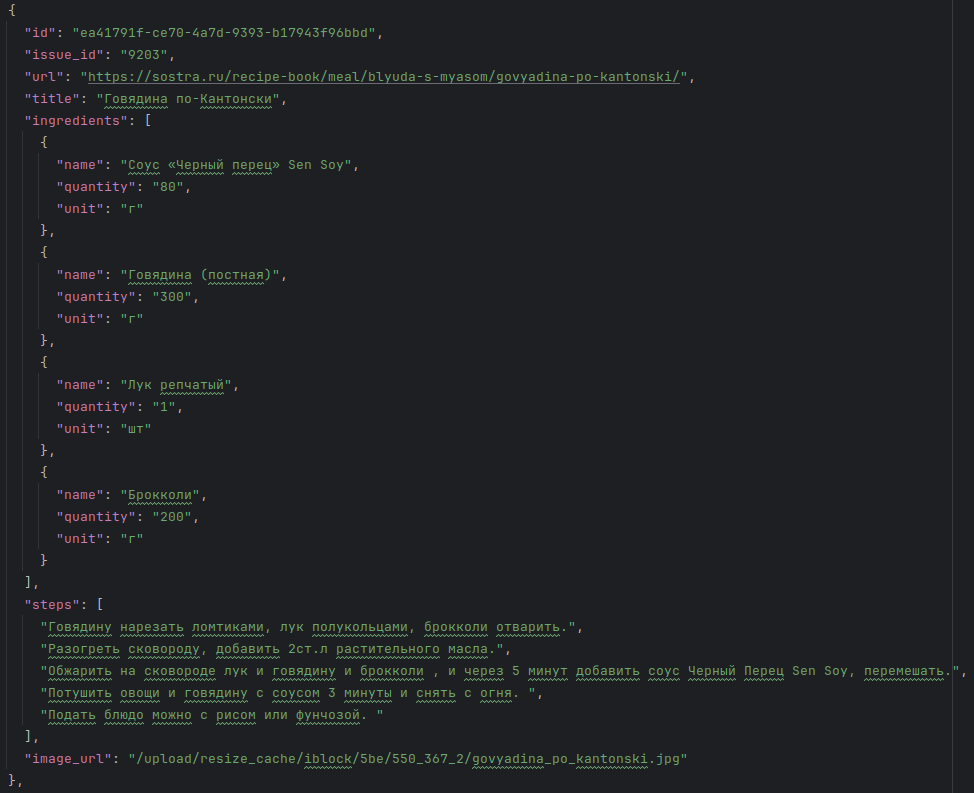
\includegraphics[width=0.5\textwidth]{test.png}
	\caption{Пример логируемых данных о задаче}
	\label{fig:test}
\end{figure} 

Все тесты были успешно пройдены.
\clearpage

\chapter{Примеры работы программы}

На рисунке~\ref{fig:json} представлен пример полученных данных. Всего получено 149 записей с данными.
\begin{figure}[H]
	\centering
	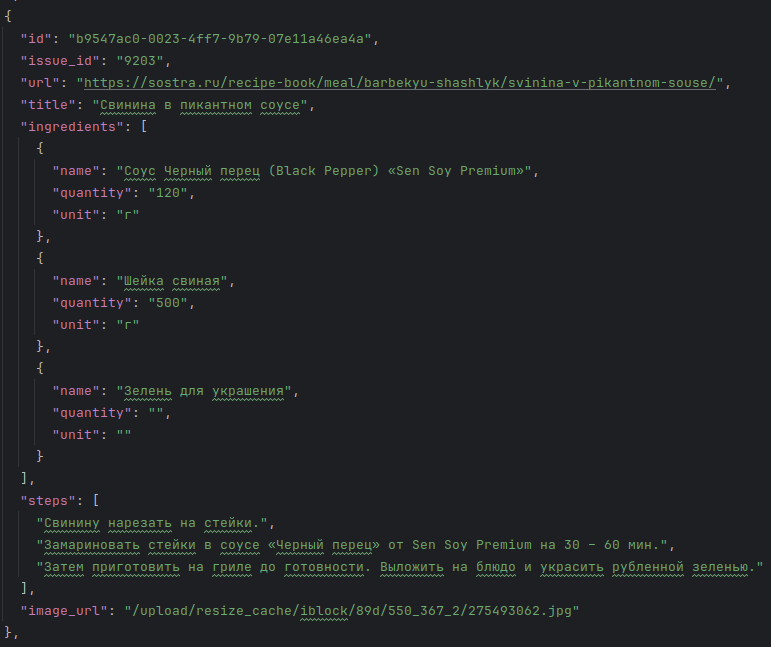
\includegraphics[width=\textwidth]{json.png}
	\caption{Данные о рецепте}
	\label{fig:json}
\end{figure}

Пример логируемых данных представлен на рисунке~\ref{fig:log}.
\begin{figure}[H]
	\centering
	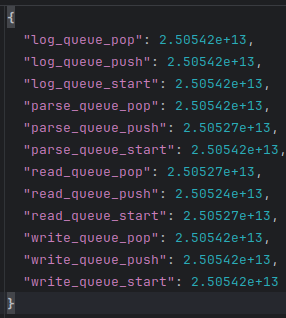
\includegraphics[width=0.5\textwidth]{log.png}
	\caption{Пример логируемых данных о задаче}
	\label{fig:log}
\end{figure}
\clearpage


\chapter{Описание исследования}

Исследования проводились на машине со следующими характеристиками:
\begin{itemize}[label=---]
	\item процессор Intel(R) Core(TM) i5-10210U, тактовая частота 1.60 ГГц;
	\item оперативная память: 16 ГБ;
	\item операционная система: Ubuntu 22.04.4 LTS.
\end{itemize}

Результаты замеров приведены в таблице~\ref{tab:all_times}.

\begin{table}[H]
	\caption{Средние времена этапов выполнения в мкс}
	\label{tab:all_times}
	\centering
	\begin{tabular}{|c|r|}
	\hline
	Среднее время существования задачи & 7805728\\\hline
	Среднее время ожидания в очереди чтения & 8645\\\hline
	Среднее время ожидания в очереди обработки & 42164\\\hline
	Среднее время ожидания в очереди записи & 14\\\hline
	Среднее время ожидания в очереди логирования & 14\\\hline
	Среднее время чтения & 208\\\hline
	Среднее время обработки & 813\\\hline
	Среднее время записи & 169\\\hline
	Среднее время логирования & 0\\\hline
	\end{tabular}
\end{table}
	
В таблице~\ref{tab:distribution} приведены метки задач, отсортированные по возрастанию времени, показывающие параллельное выполнение различных этапов конвейера.

\begin{table}[H]
	\caption{Метки задач отсортированные по возрастанию времени}
	\label{tab:distribution}
	\centering
	\begin{tabular}{|c|c|}
		\hline
		\shortstack{Время с неопределенного момента\\в прошлом в мкс} & \shortstack{Идентификатор задачи\\ и ее имя}\\\hline
		735559 & \shortstack{b01fb701-44a6-4e9d-80f2-700106696499\\read\_queue\_push}\\\hline
		742961 & \shortstack{4a91915e-5ddd-4c2f-bde9-ed82f260607a\\read\_queue\_push}\\\hline
		753717 & \shortstack{b01fb701-44a6-4e9d-80f2-700106696499\\read\_queue\_start}\\\hline
		755113 & \shortstack{b01fb701-44a6-4e9d-80f2-700106696499\\read\_queue\_pop}\\\hline
		755146 & \shortstack{b01fb701-44a6-4e9d-80f2-700106696499\\parse\_queue\_push}\\\hline
		789426 & \shortstack{79af8472-5819-4abb-834a-d56d493c693d\\read\_queue\_start}\\\hline
		790817 & \shortstack{79af8472-5819-4abb-834a-d56d493c693d\\read\_queue\_pop}\\\hline
		790860 & \shortstack{79af8472-5819-4abb-834a-d56d493c693d\\parse\_queue\_push}\\\hline
		999207 & \shortstack{b01fb701-44a6-4e9d-80f2-700106696499\\parse\_queue\_start}\\\hline
		1011835 & \shortstack{b01fb701-44a6-4e9d-80f2-700106696499\\parse\_queue\_pop}\\\hline
		1011868 & \shortstack{b01fb701-44a6-4e9d-80f2-700106696499\\write\_queue\_push}\\\hline
		1011989 & \shortstack{b01fb701-44a6-4e9d-80f2-700106696499\\write\_queue\_start}\\\hline
		1017574 & \shortstack{b01fb701-44a6-4e9d-80f2-700106696499\\write\_queue\_pop}\\\hline
		1017606 & \shortstack{b01fb701-44a6-4e9d-80f2-700106696499\\log\_queue\_push}\\\hline
		1017681 & \shortstack{b01fb701-44a6-4e9d-80f2-700106696499\\log\_queue\_start}\\\hline
		1017686 & \shortstack{b01fb701-44a6-4e9d-80f2-700106696499\\log\_queue\_pop}\\\hline
		1496252 & \shortstack{79af8472-5819-4abb-834a-d56d493c693d\\parse\_queue\_start}\\\hline
		1509341 & \shortstack{79af8472-5819-4abb-834a-d56d493c693d\\parse\_queue\_pop}\\\hline
		1509381 & \shortstack{79af8472-5819-4abb-834a-d56d493c693d\\write\_queue\_push}\\\hline
		1509502 & \shortstack{79af8472-5819-4abb-834a-d56d493c693d\\write\_queue\_start}\\\hline
		1515815 & \shortstack{79af8472-5819-4abb-834a-d56d493c693d\\write\_queue\_pop}\\\hline
		1515844 & \shortstack{79af8472-5819-4abb-834a-d56d493c693d\\log\_queue\_push}\\\hline
		1515915 & \shortstack{79af8472-5819-4abb-834a-d56d493c693d\\log\_queue\_start}\\\hline
		1516937 & \shortstack{79af8472-5819-4abb-834a-d56d493c693d\\log\_queue\_pop}\\\hline
	\end{tabular}
\end{table}
\clearpage
